\chapter{Implementing the Fault Detector}

After all the baseline foundations of deep learning and convolutional
neural networks have been derived, it is now time to apply these
methods to the problem of fault detection in the CLAS12 drift
chamber. Due to the CLAS12 productive environment heavily relying on
the JAVA ecosystem, all implementations will be carried out utilizing
the JAVA programming language as well. The basis of the autonomous
fault detection system will be formed by the deeplearning4j (DL4J)
library which will be briefly described in the following section.

\section{The Deeplearning4j Library}

Deeplearning4j is an open-source deep learning library written for the
JAVA Virtual Machine (JVM). It is supported by the well known
AI-Startup Skymind and contains implementations of many algorithms
from the artificial intelligence domain, such as convolutional neural
networks, that will be used when implementing the fault detector.

To speed up the computations that have to be performed during the
training of deep convolutional architectures, DL4J relies on its own
numerical backend engine, ND4J, that contains C++ and Cuda
implementations of all required operations, most importantly matrix
multiplications. This way, deep neural networks can be trained on
big clusters containing multiple CPUs and GPUs, leveraging the huge
amounts of parallelism introduced by these computational
architectures.

Additionally, the DL4J library also provides useful mechanisms that
make monitoring the training process highly accessible, such as
Web-UIs which offer visual representations of the loss function as
well as the weight updates during training. Evaluating the trained
classifier is also not a difficult task, as DL4J provides
designated classes that are designed to compute all the relevant
metrics on the training dataset.\footnote{See
  \url{www.deeplearning4j.org} for more information.}

\section{Data Preparation}

Before the data can be fed into a convolutional neural network, a few
steps of preparation are necessary. Recall the heatmap plots of
different faults shown in section \ref{sec:faults}. The data that will
be presented to the network will be organized in the form of a \(6
\times 112\) array representing the activation level of each wire in a
superlayer, similar to the heatmaps. This way, the spatial structure
that is present within the data is preserved, which is essential when
working with CNNs, because as shown in section \ref{sec:convnets},
these architectures heavily depend on structural assumptions on the
input. Unlike in the case of images, the fault data will only consist
of a single channel, resulting in an input volume of size \(6
\times 112 \times 1\).

Due to the fact that activation levels can vary drastically among
different sectors, sectors far away from the electron beam receiving
less particles passing by, the data has to be normalized in order to
compensate for these effects of disproportion. This is done by projecting
the activation values within each input on a numerical scale between 0
and 1, the lowest activation ending up at 0, the highest at 1. This
procedure will make it easier for the network to ignore the
differences in absolute activation levels and focus more on the local
fault patterns instead.

\section{The Fault Detection System}

When looking at the examples of various faults that can occur in the
drift chamber (see section \ref{sec:faults}), it becomes apparent that
there are usually multiple faults present within a single
superlayer (see for instance Fig. \ref{fig:dead-connector}, where
there are a dead connector as well as multiple dead wires present in a
superlayer). To account for this circumstance, multiple CNNs are
trained on the fault data, each individual CNN only specializing in
recognizing a single fault type (see section \ref{sec:faults}), thus
resulting in a binary classifier for each fault. To obtain information
on the various faults present in a single input, each individual CNN
is presented with the corresponding data. In the next step, all the
individual responses are collected, resulting in a list of faults that
were recognized within the given superlayer. The network architecture
used is similar for each CNN that is part of the fault detector as
described in the following section.

\subsection{Network Architecture and Configuration}

After the \(6 \times 112 \times 1\) input volume resulting from the
normalized activations of a superlayer, a convolution layer
is employed as the first feature extractor of the network. The layer
uses a kernel size of \(2 \times 3\) which accounts for the slightly
unsymmetrical dimensions of the input. The total number of kernels
within this layer, i.e. the amount of features to look for, is set to
20 and a stride of 1 in each direction is used. The ReLU is applied
as an activation function within this layer.
Following the convolution layer, a max-pooling layer is employed with a
filter size of \(1 \times 2\) and a stride of \(1 \times 2\) as
well. This is done in order to compress the feature data along the
``wire''-dimension. After the pooling layer, a single densely
connected hidden layer with 100 hidden neurons is inserted, utilizing
the ReLU activation function as well. The output layer consists of two
output neurons, one firing if the designated fault was detected, the
other firing if not. The softmax activation function is used on this
layer to make the ouputs interpretable as probabilities. An
illustration of the network architecture used in the fault detector
can be seen in Fig. \ref{fig:fault-architecture}.

The weights and biases of the network are initialized using the xavier
method (see section \ref{sec:xavier}), ensuring a weight distribution
that enhances network trainability. The optimization algorithm
employed is a slight variation of the traditional stochastic gradient
descent algorithm (see section \ref{sec:training}), called
ADADELTA. The advantage of this algorithm is that it is able to adjust
the learning rate during training based on the local characteristics
of the loss function, resulting in a fairly robust procedure
\cite{adadelta}. The gradients in each step of the updating process
are computed using the backpropagation algorithm (see section
\ref{sec:backpropagation}).

\begin{figure}[h]
  \centering
  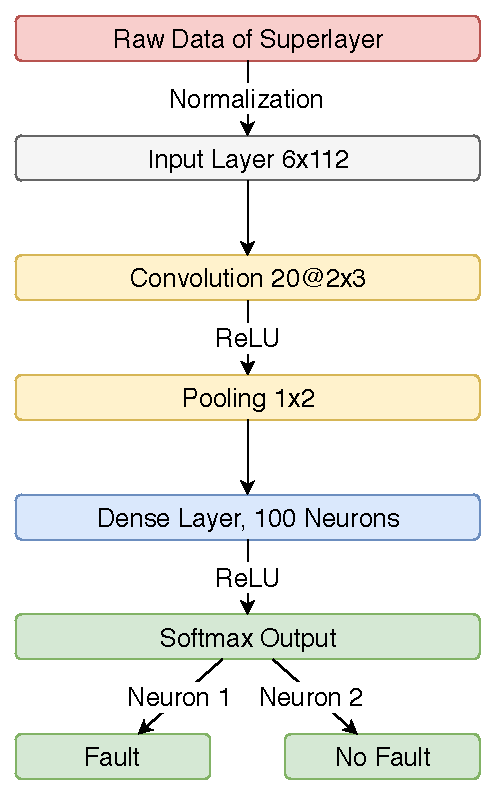
\includegraphics[height=.5\textheight]{../figures/fault_architecture}
  \caption{The architecture of a single CNN in the fault detector that
  is trained to identify a unique fault type.}
  \label{fig:fault-architecture}
\end{figure}

\section{Training the Fault Detector}

In order to train the fault detector as a whole, every single binary
CNN is trained in isolation on a collection containing an equal
balance of positive as well as negative examples of the fault type
that it is supposed to detect. The data used during training is
generated by a simulation suite that works on real fault-free heatmaps
and inserts random combinations of faults which are then labeled in
accordance and fed into the network. In order to avoid overfitting
(see section \ref{sec:classification-architecture}), the wire activations
are randomly perturbed during training, ensuring that every example
the classifier is presented with is unique.

Training a single binary classifier was not stopped until the
classification accuracy (see section
\ref{sec:classification-evaluation}) on 10.000 new random examples
reached 100\%. This procedure was repeated for every single fault
classifier. The learning curve that plots the model score against the
number of training examples of the dead wire classifier can be seen in
[TODO]. We shall see if the procedure of generating new random
examples during every training step and then training up to a 100\%
accuracy on new random data successfuly prevented overfitting and
enabled generalization when evaluating the fault detector on real
fault data.

\section{Evaluation Results}
